%% ==========================================================================
%%  dgnozzle -- nozzle geometry and boundary conditions
%%
%%  Standalone TikZ figure.  Compile on its own with
%%      pdflatex nozzle_geometry.tex
%%  or render it to the PNG that docs/theory.md shows with
%%      python docs/render_figures.py
%%
%%  The wall coordinates are the actual 'bell' contour at AR = 2.5019 and
%%  throat_x = 0.1388, sampled from dgnozzle.geometry and scaled by 12.
%%  Regenerate with:  python docs/make_tikz.py
%% ==========================================================================
\documentclass[tikz,border=6pt]{standalone}
\usepackage{amsmath}
\usetikzlibrary{arrows.meta,decorations.pathmorphing,patterns,calc,positioning}
\begin{document}

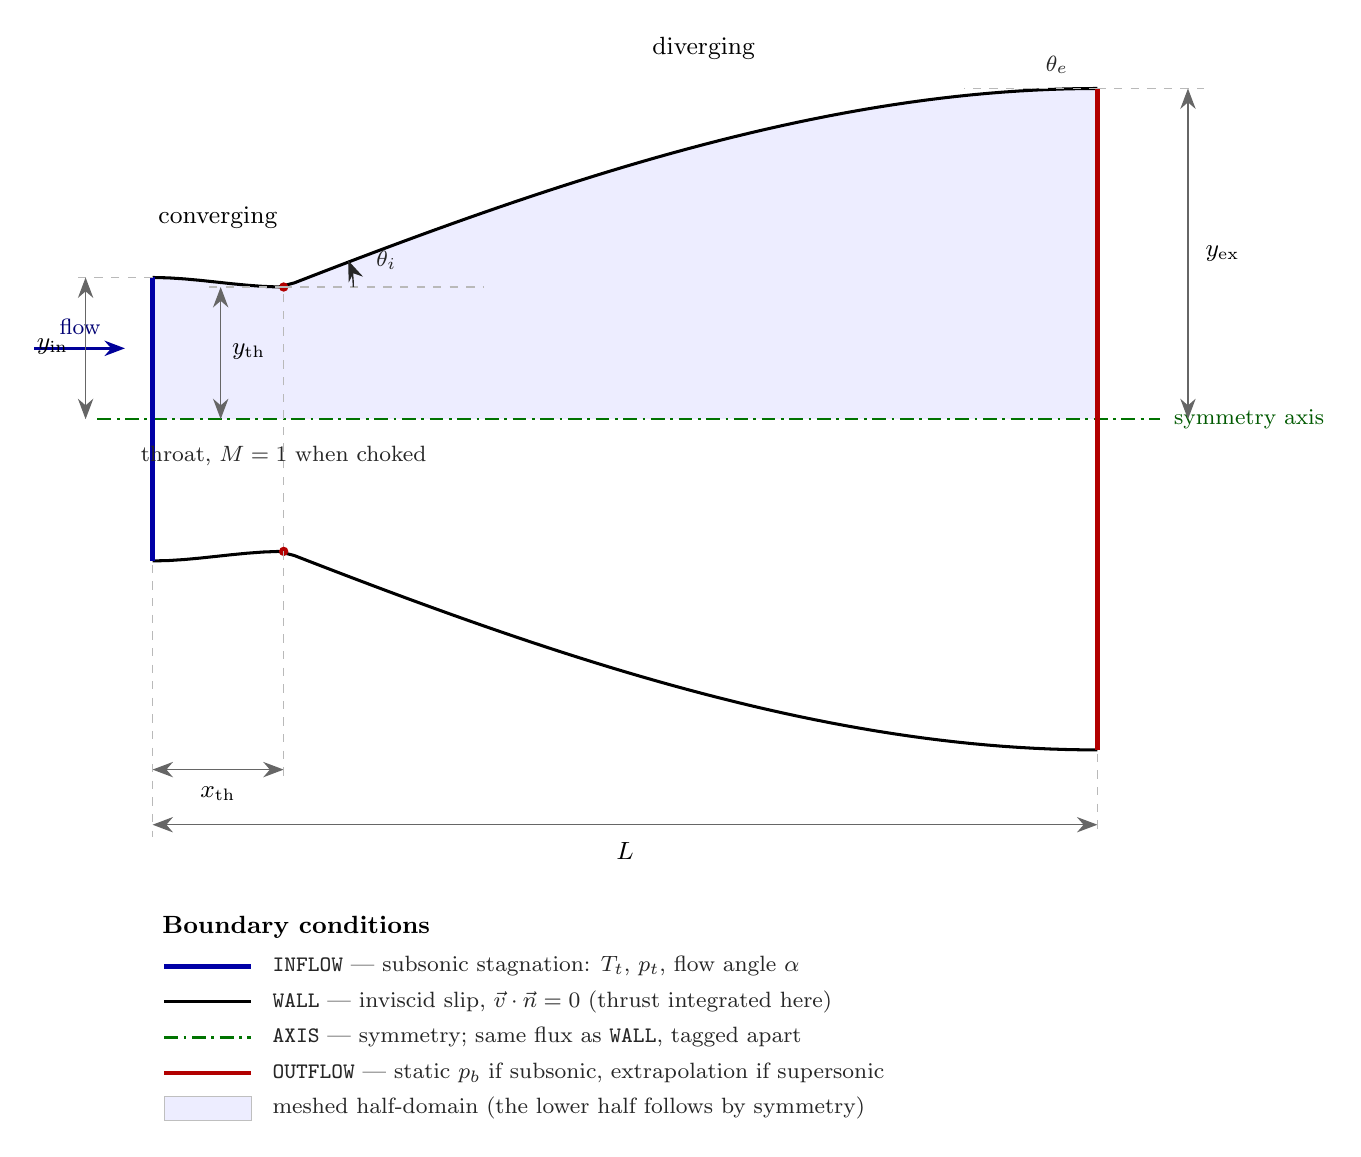
\begin{tikzpicture}[
  >={Stealth[length=2.6mm]},
  wall/.style   = {line width=1.1pt, black},
  axis/.style   = {line width=0.9pt, green!45!black, dash pattern=on 5pt off 2pt on 1pt off 2pt},
  inflow/.style = {line width=1.6pt, blue!65!black},
  outflow/.style= {line width=1.6pt, red!70!black},
  dim/.style    = {<->, gray!80!black, line width=0.5pt},
  guide/.style  = {gray!55, line width=0.4pt, dashed},
  lbl/.style    = {font=\small},
  slbl/.style   = {font=\footnotesize, gray!30!black},
]

%% ---- computational half-domain (shaded) --------------------------------
\fill[blue!7]
  plot coordinates {(0.0000,1.8000) (0.2000,1.7952) (0.4000,1.7824) (0.6000,1.7641) (0.8000,1.7429) (1.0000,1.7214) (1.2000,1.7019) (1.4000,1.6870) (1.6000,1.6793) (1.8000,1.7311) (2.0000,1.8087) (2.2000,1.8858) (2.4000,1.9625) (2.6000,2.0386) (2.8000,2.1141) (3.0000,2.1890) (3.2000,2.2633) (3.4000,2.3368) (3.6000,2.4095) (3.8000,2.4815) (4.0000,2.5526) (4.2000,2.6228) (4.4000,2.6921) (4.6000,2.7604) (4.8000,2.8277) (5.0000,2.8940) (5.2000,2.9591) (5.4000,3.0230) (5.6000,3.0858) (5.8000,3.1473) (6.0000,3.2076) (6.2000,3.2665) (6.4000,3.3240) (6.6000,3.3801) (6.8000,3.4348) (7.0000,3.4880) (7.2000,3.5396) (7.4000,3.5896) (7.6000,3.6380) (7.8000,3.6847) (8.0000,3.7297) (8.2000,3.7729) (8.4000,3.8143) (8.6000,3.8539) (8.8000,3.8915) (9.0000,3.9272) (9.2000,3.9610) (9.4000,3.9927) (9.6000,4.0223) (9.8000,4.0498) (10.0000,4.0751) (10.2000,4.0983) (10.4000,4.1192) (10.6000,4.1377) (10.8000,4.1540) (11.0000,4.1679) (11.2000,4.1793) (11.4000,4.1883) (11.6000,4.1948) (11.8000,4.1987) (12.0000,4.2000)} -- (12,0) -- (0,0) -- cycle;

%% ---- walls --------------------------------------------------------------
\draw[wall] plot coordinates {(0.0000,1.8000) (0.2000,1.7952) (0.4000,1.7824) (0.6000,1.7641) (0.8000,1.7429) (1.0000,1.7214) (1.2000,1.7019) (1.4000,1.6870) (1.6000,1.6793) (1.8000,1.7311) (2.0000,1.8087) (2.2000,1.8858) (2.4000,1.9625) (2.6000,2.0386) (2.8000,2.1141) (3.0000,2.1890) (3.2000,2.2633) (3.4000,2.3368) (3.6000,2.4095) (3.8000,2.4815) (4.0000,2.5526) (4.2000,2.6228) (4.4000,2.6921) (4.6000,2.7604) (4.8000,2.8277) (5.0000,2.8940) (5.2000,2.9591) (5.4000,3.0230) (5.6000,3.0858) (5.8000,3.1473) (6.0000,3.2076) (6.2000,3.2665) (6.4000,3.3240) (6.6000,3.3801) (6.8000,3.4348) (7.0000,3.4880) (7.2000,3.5396) (7.4000,3.5896) (7.6000,3.6380) (7.8000,3.6847) (8.0000,3.7297) (8.2000,3.7729) (8.4000,3.8143) (8.6000,3.8539) (8.8000,3.8915) (9.0000,3.9272) (9.2000,3.9610) (9.4000,3.9927) (9.6000,4.0223) (9.8000,4.0498) (10.0000,4.0751) (10.2000,4.0983) (10.4000,4.1192) (10.6000,4.1377) (10.8000,4.1540) (11.0000,4.1679) (11.2000,4.1793) (11.4000,4.1883) (11.6000,4.1948) (11.8000,4.1987) (12.0000,4.2000)};
\draw[wall] plot coordinates {(0.0000,-1.8000) (0.2000,-1.7952) (0.4000,-1.7824) (0.6000,-1.7641) (0.8000,-1.7429) (1.0000,-1.7214) (1.2000,-1.7019) (1.4000,-1.6870) (1.6000,-1.6793) (1.8000,-1.7311) (2.0000,-1.8087) (2.2000,-1.8858) (2.4000,-1.9625) (2.6000,-2.0386) (2.8000,-2.1141) (3.0000,-2.1890) (3.2000,-2.2633) (3.4000,-2.3368) (3.6000,-2.4095) (3.8000,-2.4815) (4.0000,-2.5526) (4.2000,-2.6228) (4.4000,-2.6921) (4.6000,-2.7604) (4.8000,-2.8277) (5.0000,-2.8940) (5.2000,-2.9591) (5.4000,-3.0230) (5.6000,-3.0858) (5.8000,-3.1473) (6.0000,-3.2076) (6.2000,-3.2665) (6.4000,-3.3240) (6.6000,-3.3801) (6.8000,-3.4348) (7.0000,-3.4880) (7.2000,-3.5396) (7.4000,-3.5896) (7.6000,-3.6380) (7.8000,-3.6847) (8.0000,-3.7297) (8.2000,-3.7729) (8.4000,-3.8143) (8.6000,-3.8539) (8.8000,-3.8915) (9.0000,-3.9272) (9.2000,-3.9610) (9.4000,-3.9927) (9.6000,-4.0223) (9.8000,-4.0498) (10.0000,-4.0751) (10.2000,-4.0983) (10.4000,-4.1192) (10.6000,-4.1377) (10.8000,-4.1540) (11.0000,-4.1679) (11.2000,-4.1793) (11.4000,-4.1883) (11.6000,-4.1948) (11.8000,-4.1987) (12.0000,-4.2000)};

%% ---- symmetry axis ------------------------------------------------------
\draw[axis] (-0.7,0) -- (12.8,0);
\node[slbl, green!35!black, anchor=west] at (12.85,0) {symmetry axis};

%% ---- inflow and outflow planes -----------------------------------------
\draw[inflow]  (0,0) -- (0,1.8000);
\draw[inflow]  (0,0) -- (0,-1.8000);
\draw[outflow] (12,0) -- (12,4.2000);
\draw[outflow] (12,0) -- (12,-4.2000);

%% ---- flow direction -----------------------------------------------------
\draw[->, blue!60!black, line width=0.9pt] (-1.5,0.9) -- (-0.35,0.9);
\node[slbl, blue!45!black, anchor=south] at (-0.92,0.95) {flow};

%% ---- throat -------------------------------------------------------------
\draw[guide] (1.6656,-1.6787) -- (1.6656,1.6787);
\fill[red!70!black] (1.6656,1.6787) circle (1.7pt);
\fill[red!70!black] (1.6656,-1.6787) circle (1.7pt);

%% ---- dimensions ---------------------------------------------------------
\draw[guide] (0,1.8000) -- (-1.05,1.8000);
\draw[dim]   (-0.85,0) -- (-0.85,1.8000);
\node[lbl, anchor=east] at (-0.95,0.92) {$y_{\mathrm{in}}$};

\draw[guide] (1.6656,1.6787) -- (0.6656,1.6787);
\draw[dim]   (0.8656,0) -- (0.8656,1.6787);
\node[lbl, anchor=west] at (0.8856,0.86) {$y_{\mathrm{th}}$};

\draw[guide] (12,4.2000) -- (13.35,4.2000);
\draw[dim]   (13.15,0) -- (13.15,4.2000);
\node[lbl, anchor=west] at (13.25,2.1) {$y_{\mathrm{ex}}$};

\draw[dim] (0,-5.15) -- (12,-5.15);
\node[lbl, anchor=north] at (6,-5.25) {$L$};
\draw[dim] (0,-4.45) -- (1.6656,-4.45);
\node[lbl, anchor=north] at (0.83,-4.55) {$x_{\mathrm{th}}$};
\draw[guide] (0,-1.85) -- (0,-5.3);
\draw[guide] (1.6656,-1.6787) -- (1.6656,-4.6);
\draw[guide] (12,-4.25) -- (12,-5.3);

%% ---- wall angles --------------------------------------------------------
\draw[guide] (1.6656,1.6787) -- (4.2,1.6787);
\draw[->, gray!30!black, line width=0.5pt] (2.55,1.6787) arc (0:22:0.9);
\node[slbl, anchor=west] at (2.72,2.02) {$\theta_i$};

\draw[guide] (12,4.2000) -- (10.3,4.2000);
\node[slbl, anchor=south east] at (11.75,4.26) {$\theta_e$};

%% ---- region labels ------------------------------------------------------
\node[lbl, anchor=south] at (0.83,2.30) {converging};
\node[lbl, anchor=south] at (7.0,4.45)  {diverging};
\node[slbl, anchor=north] at (1.6656,-0.22) {throat, $M = 1$ when choked};

%% ---- boundary-condition legend -----------------------------------------
\begin{scope}[shift={(0,-7.4)}]
  \node[lbl, anchor=west] at (0,0.95) {\textbf{Boundary conditions}};
  \draw[inflow]  (0.15,0.45) -- (1.25,0.45);
  \node[slbl, anchor=west] at (1.4,0.45)
    {\texttt{INFLOW} --- subsonic stagnation: $T_t$, $p_t$, flow angle $\alpha$};
  \draw[wall]    (0.15,0.00) -- (1.25,0.00);
  \node[slbl, anchor=west] at (1.4,0.00)
    {\texttt{WALL} --- inviscid slip, $\vec{v}\cdot\vec{n} = 0$ (thrust integrated here)};
  \draw[axis]    (0.15,-0.45) -- (1.25,-0.45);
  \node[slbl, anchor=west] at (1.4,-0.45)
    {\texttt{AXIS} --- symmetry; same flux as \texttt{WALL}, tagged apart};
  \draw[outflow] (0.15,-0.90) -- (1.25,-0.90);
  \node[slbl, anchor=west] at (1.4,-0.90)
    {\texttt{OUTFLOW} --- static $p_b$ if subsonic, extrapolation if supersonic};
  \fill[blue!7] (0.15,-1.50) rectangle (1.25,-1.20);
  \draw[gray!50, line width=0.3pt] (0.15,-1.50) rectangle (1.25,-1.20);
  \node[slbl, anchor=west] at (1.4,-1.35)
    {meshed half-domain (the lower half follows by symmetry)};
\end{scope}

\end{tikzpicture}

\end{document}
